\documentclass{article}
\usepackage[utf8]{inputenc}
\usepackage{geometry}
\usepackage{graphicx}
\usepackage{url,hyperref}
\usepackage{float}
\usepackage[bottom]{footmisc}
\usepackage{fancyvrb}
\usepackage{textcomp}
\hypersetup{
	colorlinks = true,
	citecolor = green,
	urlcolor = cyan
}

\title{
	Web Information Extraction and Retrieval\\
	Programming Assignment 2: \\
	Document Parsing
}
\author{
	Marko Prelevikj\\
	63130345\\
	\texttt{mp2638@student.uni-lj.si}
	\and
	Gojko Hajduković\\
	63180431\\
	\texttt{gh8590@student.uni-lj.si}
	\and
	Stefan Ivanišević\\
	63170405\\
	\texttt{si0539@student.uni-lj.si}
}
\date{May 2019}

\begin{document}
	
	\maketitle
	
	\section{Introduction}
	Nowadays, \texttt{World Wide Web} represents an inexhaustible source of information with its size constantly and rapidly enlarging from day to day. Most of the pages that the \texttt{WWW} consists of are pages created according to some predefined, structured layout. Extraction of data from the Web pages is very useful and widely used today in many applications for all sorts of purposes from web scraping, web and data mining to all sorts of monitoring such as weather data monitoring, real-estate listing, price comparisons, etc. In this paper we introduce three different approaches in structured data extraction (\textit{Regular expressions, Xpath queries} and \textit{RoadRunner}) from three different types of web pages(\textit{\href{https://www.overstock.com/}{Overstock.com}, \href{https://www.rtvslo.si/}{RtvSlo.si}} and \textit{\href{http://www.autodiler.me}{Autodiler.me}}). Explanation and implementation specifics are provided in following sections.\footnotemark
	\footnotetext{Data is available on our \href{https://github.com/pr3mar/ieps-parser}{GitHub repository}, alongside with source code and results from our implementations.}
	
	\section{Chosen web page}
	For our web site of choice, we have picked the \href{http://www.autodiler.me}{audodiler.me} web page. From this web site, we have a page representing a  \href{http://www.autodiler.me/auto_oglasi_auto}{car} query and another one for \href{http://www.autodiler.me/auto_oglasi_kamion}{trucks}. The pages are  downloaded and made available for offline reading i.e. extracting within the \textit{inputs} folder. Data (e.g. "Name", "Date", "Year made", etc.) that we are going to extract from the above-mentioned pages is presented in Figure~\ref{fig:adiler}.
	
	\begin{figure}[H]
		\centering
		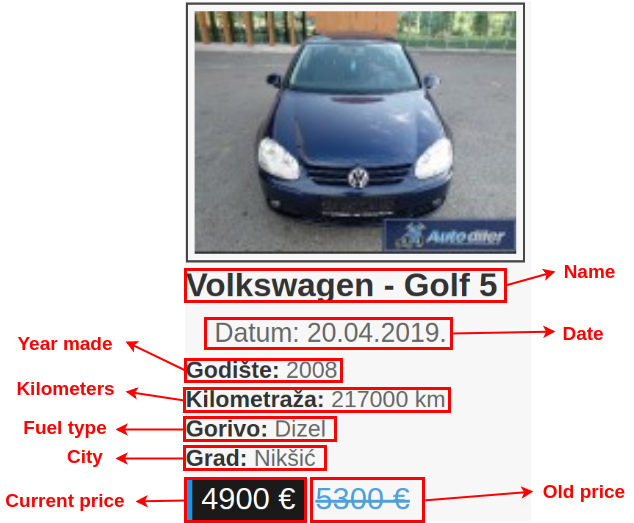
\includegraphics[width=8cm]{adiler.png}
		\caption{AutoDiler.me Web page sample}
		\label{fig:adiler}
	\end{figure}
	
	\section{Regular Expression}
	A regular expression is a string of text that allows us to create patterns that help match, search, and manipulate text. Regex is very helpful when having to parse a large amount of text. In our example, for extracting predefined data from the HTML pages we have used a regex that are defined bellow.
	\subsection{Overstock.com}
	\texttt{Overstock} represent a "listing" type of Web page, having many data records that have the same layout. The regular expression used for extracting data items for a data record is:    
	\begin{Verbatim}
	[\d\-kKt]{5}.*?)<\/b>|
	<s>(.*?)<\/s>|
	<span class=\"bigred\"><b>(\$\d*,*\d+.\d+)</b></span>|
	<span class=\"littleorange\">(\$\d*,*\d+.\d+)*\s\((\d+\%)\)</span>|
	<span class=\"normal\">\s*(.*?)\s*<br>
	\end{Verbatim}
	Extraction of data is done using a single regular expression using multiple logical \textit{OR}s. We did this to illustrate the power of regular expressions. This approach of extracting data is much shorter but it's not as readable as the next two approaches we used. 
	
	\subsection{RtvSlo.si}
	Regular expressions used for extracting data items from the \texttt{RtvSlo} web pages are:
	\begin{itemize}
		\item \textbf{Author} - \verb|<div class=\"author-name\">(.*?)<\/div>|
		\item \textbf{Published Time} - \verb|<div class=\"publish-meta\">[\n\s]*(.*?)<br>|
		\item \textbf{Title} - \verb|<h1>(.*)<\/h1>| 
		\item \textbf{Subtitle} - \verb|<div class=\"subtitle\">(.*?)<\/div>|
		\item \textbf{Lead} - \verb|<p class=\"lead\">(.*?)<\/p>|
		\item \textbf{Content} - \verb|<article.*?<p.*?>(.+)<\/p>.*<\/article>|
	\end{itemize}
	
	\subsection{AutoDiler.me}
	Regular expressions used for extracting data items for a data record from a \texttt{Autodiler} web pages shown in Figure~\ref{fig:adiler} are:
	\begin{itemize}
		\item \textbf{Name} - \verb|<h1>.*?>(.*?)<|
		\item \textbf{Image} - \verb|<div class=\"oglas_thumb.*?\">.*?<img src=\"(.*?.jpg)\"|
		\item \textbf{Date} - \verb|Datum: ([\d\.]+)*\.|
		\item \textbf{Year} - \verb|Godi.*?te:</strong> <span>(\d{4})|
		\item \textbf{Kilometers} - \verb|Kilometra.*?a:</strong> <span>(\d+)|
		\item \textbf{Fuel} - \verb|Gorivo:</strong> <span>(\w+)<| 
		\item \textbf{City} - \verb|Grad:</strong> <span>(.*?)<|
		\item \textbf{Current price and Old price} - \verb|<div class=\"priceWrapper\"><span class=\"|
		\verb|currentPrice\">(\d+ \€)(<\/span><span class=\"oldPrice\">(\d+ \€)<\/span|
		\verb|><\/div>)*"|
	\end{itemize}
	
	\section{Xpath}
	As one of the approaches in extracting structured data from Web pages we used XML path language, \texttt{Xpath}. Xpath represents a query/path language that is mainly used for finding any element on the Web page based on traversing a tree representation of XML document. We have converted HTML document to a XML document in order to make it accessible for \texttt{Xpath} usage.
	\textit{Absolute} and \textit{relative} \texttt{Xpath} queries are available and used. Even though, absolute \texttt{Xpath} queries are faster, since it is a direct path from the root of a tree to an element,adding or removing an element in the tree makes \texttt{Xpath} query fail. In this project we have used relative \texttt{Xpath} queries.
	
	\subsection{Overstock.com}
	\texttt{Overstock} represent a "listing" type of Web page, having many data records that have a same layout. \texttt{Xpath} queries used for extracting data items for a data record are:
	\begin{itemize}
		\item \textbf{Title} - \texttt{'//a/b[contains(text(),"-kt") or contains(text(),"-Kt") ]/text()'} 
		\item \textbf{List price} - \texttt{'//td[b[contains(text(),"List Price:")]]/following-sibling::td//text()'} 
		\item \textbf{Price} - \texttt{'//td[b[text()="Price:"]]/following-sibling::td//text()'} 
		\item \textbf{Saving(percent)} - \texttt{'//td[b[text()="You Save:"]]/following-sibling::td//text()'} 
		\item \textbf{Content}  -\texttt{'//td[span[@class="normal"]]/span/text()'} 
	\end{itemize}
	
	\subsection{RtvSlo.si}
	Xpath queries used for extracting data items from a \texttt{RtvSlo} web pages are :
	\begin{itemize}
		\item \textbf{Author} - \texttt{'//*[@class="author-name"]//text()'}  
		\item \textbf{Published Time} - \texttt{'//*[@class="publish-meta"]//text()'} 
		\item \textbf{Title} - \texttt{'//*[contains(@class,"news-container")]//header//h1//text()'}  
		\item \textbf{Subtitle} - \texttt{'//*[contains(@class,"news-container")]//header//div[@class="subtitle"]//text()'}  
		\item \textbf{Lead} - \texttt{'//*[contains(@class,"news-container")]//header//p[@class="lead"]//text()'}  
		\item \textbf{Content} - \texttt{'//div[contains(@class,"article-body")]//p//text()'} 
	\end{itemize}
	
	\subsection{AutoDiler.me}
	\texttt{Xpath} queries used for extracting data items for a data record from a \texttt{Autodiler} pages shown in Figure~\ref{fig:adiler} are:
	\begin{itemize}
		\item \textbf{Name} - \texttt{'//*[contains(@class,"oglas\_thumb")]/div[2]//h1//text()'} 
		\item \textbf{Image} - \texttt{'//*[contains(@class,"oglas\_thumb")]/div[1]//img//@src'}
		\item \textbf{Date} - \texttt{'//*[contains(@class,"oglas\_thumb")]/div[3]//span[@class="date"]//text()'} 
		\item \textbf{Year} - \texttt{'//*[contains(text(),"Godište")]/following-sibling::span/text()'} 
		\item \textbf{Kilometres} - \texttt{'//*[contains(text(),"Kilometr")]/following-sibling::span/text()'} 
		\item \textbf{Fuel} - \texttt{'//*[contains(text(),"Gorivo")]/following-sibling::span/text()'}  
		\item \textbf{City} - \texttt{'//*[contains(text(),"Grad")]/following-sibling::span/text()'} 
		\item \textbf{Current price} - \texttt{'//div[contains(@class,"priceWrapper")]/span[1]/text()'} 
		\item \textbf{Old price} - \texttt{'//div[contains(@class,"priceWrapper")]/span[2]/text()'} 
	\end{itemize}
	
	\section{Road Runner}
	A more automated way of extracting data is using more advanced method, such as \textit{RoadRunner}~\cite{crescenzi2001roadrunner}. The purpose of this method is to generate a \textit{wrapper} which is going to include all the data fields which contain data, and will ease the extraction of the data in the future. \textit{RoadRunner} is an approach which takes a reference page as a wrapper, and compares it to the rest of the pages from a single domain, and tries to build a wrapper.
	
	We have two different approaches on how to implement a \textit{RoadRunner}-like algorithm. One is based on basic string matching, without using a special data structure for recursive moving along the document and it will produce a regex-like output, and another one which uses a tree-like structure provided by \texttt{JSoup}~\cite{jsoup}.
	
	\subsection{Version 1}\label{v1}
	
	First version that we have tried to build of a RoadRunner like algorithm is based on a RoadRunner description~\cite{crescenzi2001roadrunner} and it is mostly working with lists and matching list elements (\texttt{HTML} tokens). We will neglect pseudo-code for this algorithm and just provide the description of the algorithm and problem that we have encounter during this implementation.
	
	\subsubsection{Prepocessing and matching}
	From the two input \texttt{HTML} files we remove \texttt{<head>} tag and everything in it and also we remove all \texttt{<script>s} and all comments from the code. Everything is in lowercase and we transfer them into \texttt{.xml} files using \texttt{BeautifulSoup}~\cite{BeautifulSoup} module, which will help us with semi-structured \texttt{HTML} files\footnote{Since some \texttt{HTML} files can have some enclosed tags, this process in our preprocessing steps will help us to avoid further problems with this type of tags.}. 
	
	After preprocessing we have two lists created from two input \texttt{HTMLs} (wrapper list and sample list, respectively), with elements that are tokens from the input \texttt{HTML} files. This tokens can be HTML tags with attributes or some text, and based on that we continue with matching the corresponding element of the wrapper with the corresponding element of the sample list. While matching list elements there will occur mismatches. We can have two types of mismatch, \textit{string mismatch} and \textit{tag mismatch}. 
	
	\subsubsection{Algorithm overview}
	When we discover that a token is a string we change it to \texttt{\#PCDATA} and continue with next element. This method we also use when we encounter a \textit{string mismatch}, we change both strings to \texttt{\#PCDATA} and continue with matching next elements.  
	On the other hand, if \textit{tag mismatch} happens we explore two options that can be a cause to this mismatch. 
	First option that we consider when \textit{tag mismatch} happens is that a mismatch is due to the iterators (which we denote as \texttt{(iterator)+}. During this process of discovering iterators we are looking for terminal tags and initial tags of an iterator. If we find them, we know that that mismatch is due to the iterator and we proceed with finding iterators. This is done recursively since more mismatches can occur during matching inner tokens of the iterator. 
	Other \textit{tag mismatch} can be optional which we denote as \texttt{(iterator)?}. Optional mismatches are easier to find, since they can happen only on wrapper or on sample, not on both of them at the same. We do this by looking for a wrapper tag on a sample page and if we do not find it then we know that a wrapper tag is optional. Similarly, we are looking for sample tag, just instead of finding for it on a sample page we are searching wrapper page. 
	
	\subsubsection{Problem}
	The problem that we encountered during the execution of our algorithm is writing the data in the output file. If our algorithm never goes into recursion, everything will work smoothly, but as soon as recursion starts, our way of writing iterators and optional tags in output starts to create problems. Since we are writing mismatches as soon as we find them, and since we are looking for optional tags only when the search for iterators fails, that means that recursion will search for the optional tags last if it finds them then recursion will write them as first in the output.
	
	\subsubsection{Output}
	Output is regex-like expression which consists of a \texttt{HTML} tags, \texttt{\#PCDATA} which are strings, iterators \texttt{+} and optional tags \texttt{?}. 
	For output files, which can be found in /outputs/road\_runner\v1 folder, to be more human readable we prettify it using BeautifulSoup. It can be opened as \texttt{HTML} file in any browser, but we recommend that it is opened in text editor for easier readability.
	
	\subsection{Version 2}\label{v2}
	This approach is consisted of a preprocessing step, similar to the one described in Section~\ref{v1}  in which we clear out all the attributes from all \textit{HTML} tags, apart from the links \texttt{<a></a>}, and images \texttt{<img/>}, from the input pages. We do all the preprocessing using \texttt{Jsoup}, and as a consequence we get a recursive structure of the \textit{HTML} pages. Next up is the building of the wrapper, which we further discuss in Subsection~\ref{v2-pseudo}. The core principles of this approach lie within the comparison of the nodes, and how we expand the wrapper.
	
	\subsubsection{Pseudo code} \label{v2-pseudo}
	Following the preprocessing, we do the  steps:
	\begin{enumerate}
		\item Pick a random page as a reference page, i.e. wrapper, and use the other page to compare the wrapper to.
		\item We compare the pages level by level, recursively:
		\begin{itemize}
			\item compare the current wrapper tag to the other tag (described below)
			\item if they are an exact match, we have detected static content and we add it to the wrapper
			\item if there are mismatches, we continue the comparison recursively
			\item finally, compare the leaves and mark the nodes as data nodes
		\end{itemize}
		\item Return the result as a final wrapper.
	\end{enumerate}
	
	\subsubsection{Comparison function}
	The comparison is the most important information we get to make our decision on what to do in the recursion next. As a result from it, we get a list denoting whether the nodes are:
	\begin{itemize}
		\item equal tag name, if not - continue
		\item equal number of children, if yes - it is a potential candidate for an iterator
		\item shared tag name among children, if yes - it is most likely an iterator
		\item equal text contained within them, if yes - it is static content
		\item equal link/image attributes, if not - the link/image content is dynamic
	\end{itemize}
	With the comparison function we detect the static and dynamic contents of the page, the multiple items which are equal (referred to as \textit{iterator}), and if there are heterogeneous child nodes (i.e. their tag names do not match) we handle them separately.
	
	\subsubsection{Building the wrapper}
	The task of building the wrapper is performed based on the properties obtained from the comparison function. We have a trivial case when the detected content is an exact match between the pages, in which we add the content to the wrapper, and continue with the processing. Another rather trivial case is when we need reach the leaf tags which have dynamic content and we need to generalize the node. 
	
	More troublesome cases are handling the iterators and the heterogeneous lists. In the case of iterators, we need to expand the same \textit{HTML} tag to contain all the properties from every item in the iterator. We do that by comparing the elements and expanding the generic tag element which is the wrapper element. This way we ensure that all of the elements are processed and included in the final wrapper.
	
	When dealing with the heterogeneous lists, we cannot compare nodes which are of different type (different tag names). So, in order to overcome this problem, we are using a method which zips\footnote{creates a list of pairs of nodes which are of same type, and leaves the mismatched elements as pairs with empty elements} the nodes heuristically: matching the nodes by their node tags greedily, i.e. assuming that the nodes which are of same type are a part of an iterator, and leaving the unmatched ones as singles which expand the wrapper independently.
	
	\subsubsection{Node generalization}
	A node which is detected to have dynamic content, is generalized by removing all the text within it, and its children, and has generalized data such as:
	\begin{itemize}
		\item empty text is generalized to \texttt{\$data}
		\item class \texttt{optional} is added to the generalized node
		\item links are generalized to \texttt{<a href="\$link">\$link-data</a>}
		\item images are generalized to \texttt{<img src="\$img-link" alt="\$img-alt">}
	\end{itemize}
	
	\subsubsection{Output}
	The output is in the form of a generalized \textit{HTML} page which has the generalized nodes as data holders. With this output we are preserving all the static content of the page, and we mark the places where the dynamic content is.
	
	In its raw form, i.e. text, the wrapper is also in a human readable form, as the wrapper can be opened in a web browser of choice. For more clarity on the wrappers' attributes we advise to be opened in a text editor, as the output is prettified using \texttt{JSoup}, and it allows the reader a convenient experience while reading the \textit{HTML} code.
	
	\subsubsection{Results}
	As a guideline for our implementation of this approach we used a simple example\footnote{included in the input files in our \href{https://github.com/pr3mar/ieps-parser}{GitHub repository}}, which was presented at our lectures, which we further extended to cover all of the edge cases which may occur.
	
	Additionally, we analyzed the input pages, and concluded that some of them (RtvSlo.si pages) have some inconsistencies within them, which our implementation does not cover, and thus is under-performing. The inconsistency is consisted of some \texttt{div} tags being mis-aligned which makes our naive approach crash, as it violates the first and most important assumption that the tags with matching names lying on the same level and position are equal elements.
	
	The rest of the websites are rather consistent, which means that our approach performs rather well on the rest of the pages. We can conclude this by simply comparing the wrapper sizes (number of lines in the \texttt{.html} file) to the size of the original pages. As an example, the \texttt{AutoDiler.me} websites perform the best, as our approach managed to match most of the content and generalize it really well.
	
	On the other hand, the wrapper for \texttt{RtvSlo.si} is bigger than the original pages, which indicates that there is something wrong with our algorithm, as we are trying to minimize, i.e. generalize, the content from pages which we know are similar.
	
	\section{Conclusion}
	In this paper we have introduced three different approaches in structured data extraction from the web pages. We first present two approaches , \texttt{XPath} and \texttt{Regular Expressions} that are still currently widely used in structured data extraction. Both of the previously explained approaches have their shortcomings in the sense that those are manual approaches that for large companies require a lot of labor resources. As for our third approach we introduce two versions of the \texttt{RoadRunner}-like implementation which represents the automated way of generating a wrapper for data extraction.
	
	
	\bibliographystyle{IEEEtran}
	\bibliography{refs}
	
\end{document}
